\section{Batteries}

\begin{multicols}{2}
{\small 	\textbf{Pb Batteries} 
	\begin{equation*}
		Pb + PbO_2 + 2H_2SO_4 \Leftrightarrow 2PbSO_4 + 2H_2O
	\end{equation*}
	
	\begin{itemize}
		\setlength{\itemsep}{0pt}
		\item[+] Low price due to high number of pieces
		\item[+] Available in many different types
		\item[+] Well recyclable
		\item[-] Slight specific energy
		\item[-] Not allowed for deep discharging
		\item[-] Low lifespan and temp. sensitive
	\end{itemize}
	
	\textbf{NiCd}
	\begin{equation*}
		2NiOOH + Cd + 2H_20 \Leftrightarrow 2Ni(OH)_2 + Cd(OH)_2
	\end{equation*}
	
	\begin{itemize}
		\setlength{\itemsep}{0pt}
		\item[+] High power, fast-chargeable (0.1 - 4C)
		\item[+] Low temperature compatibility
		\item[+] High number of cycles (1000 - 4000)
		\item[-] Temperature sensitive
		\item[-] Memory effect
		\item[-] Highly self-discharging rate
	\end{itemize}
	
	\textbf{NiMH}
	\begin{equation*}
		NiOOH + MeH \Leftrightarrow Ni(OH)_2 + Me
	\end{equation*}

	\begin{itemize}
		\setlength{\itemsep}{0pt}
		\item[+] High energy density
		\item[+] Fast chargeable
		\item[+] Low costs and ecological
		\item[-] Low power density
		\item[-] Memory effect
		\item[-] High self-discharging rate
	\end{itemize}
	
	\textbf{Lithium Ion Batteries}
	
	\begin{itemize}
		\setlength{\itemsep}{0pt}
		\item[+] High voltage $U = 3.6~V$
		\item[+] High specific energy density
		\item[+] High discharge current of 10C
		\item[-] low thermal stability
		\item[-] rather expensive
		\item[-] charging is complicated
	\end{itemize}}	
	
\end{multicols}


\begin{multicols}{3}
\subsection{Peukert factor}
	Peukert factor $k$; $1.1 (better) < k < 1.5$: 
	\begin{equation*}
		H_x = H_0 \cdot \left(\frac{H_0}{T_0 \cdot I_x}\right)^{k-1}
	\end{equation*}	
	\begin{equation*}
		I_k \cdot t_e = C
	\end{equation*}
	\\ \\ \\
{\footnotesize 	\begin{tabbing}
		$I_k$: \hspace{0.1cm} \= Peukert corrected discharge current \\
		$t_e$: \> discharge time \\
		$C$: \> constant \\
		$H_x$: \> available capacity \\
		$I_x$: \> applied current \\
		$H_0$: \> manufacturer's capacity value [Ah] \\
		\> corresponding to the discharge time $T_0$ [h]
	\end{tabbing}}


\subsection{ESR}
Take highest ($I_1$) and lowest ($I_2$) current curve and determine corresponding voltage points ($U_{11}$ and $U_{12}$).
\begin{equation*}
	R_{ESR} = \frac{U_{12} - U_{11}}{I_1 - I_2}
\end{equation*}

\end{multicols}

\subsection{Modelling}
\begin{minipage}[lt]{7cm}
	\centering
	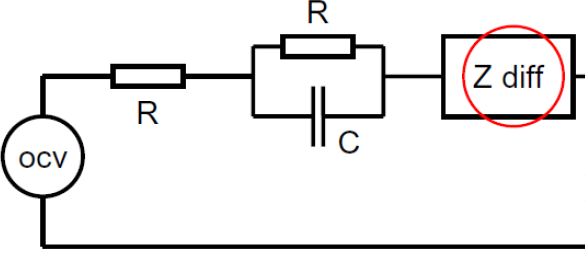
\includegraphics[width=0.7\textwidth]{./images/Battery_modelling.png}
\end{minipage}
\begin{minipage}[rt]{10cm}
	The aging process is simulated with $Z_{diff}$. One possible calculation for this impedance is the so called Warburg impedance (semi-infinite diffusion).
	\begin{equation*}
		Z\left(\omega\right) = \frac{K}{\sqrt{j\omega}} = \frac{K \left(1-j\right)}{\sqrt{2\omega}}
	\end{equation*}
\end{minipage}
